\section{Language Extensions}
\label{sec:extension}

This section formalizes extensions of the target language of
verification.  Our approach is to translate a source program to a
program that has no recursive data structures and no control operators.
The translation is sound and complete.

Figure~\ref{fig:extension} shows the verification framework for recursive data structures and control
operators.
%\begin{enumerate}
% \item Translation of a source program with control operations into a
%       program with no control operations.
% \item Translation of a program with recursive data structures into a program with lists.
% \item Translation of the program with lists into a program with integers.
% \item Verification for higher-order programs with integers based on our previous framework.
%\end{enumerate}

\begin{figure}[t]
 \begin{center}
  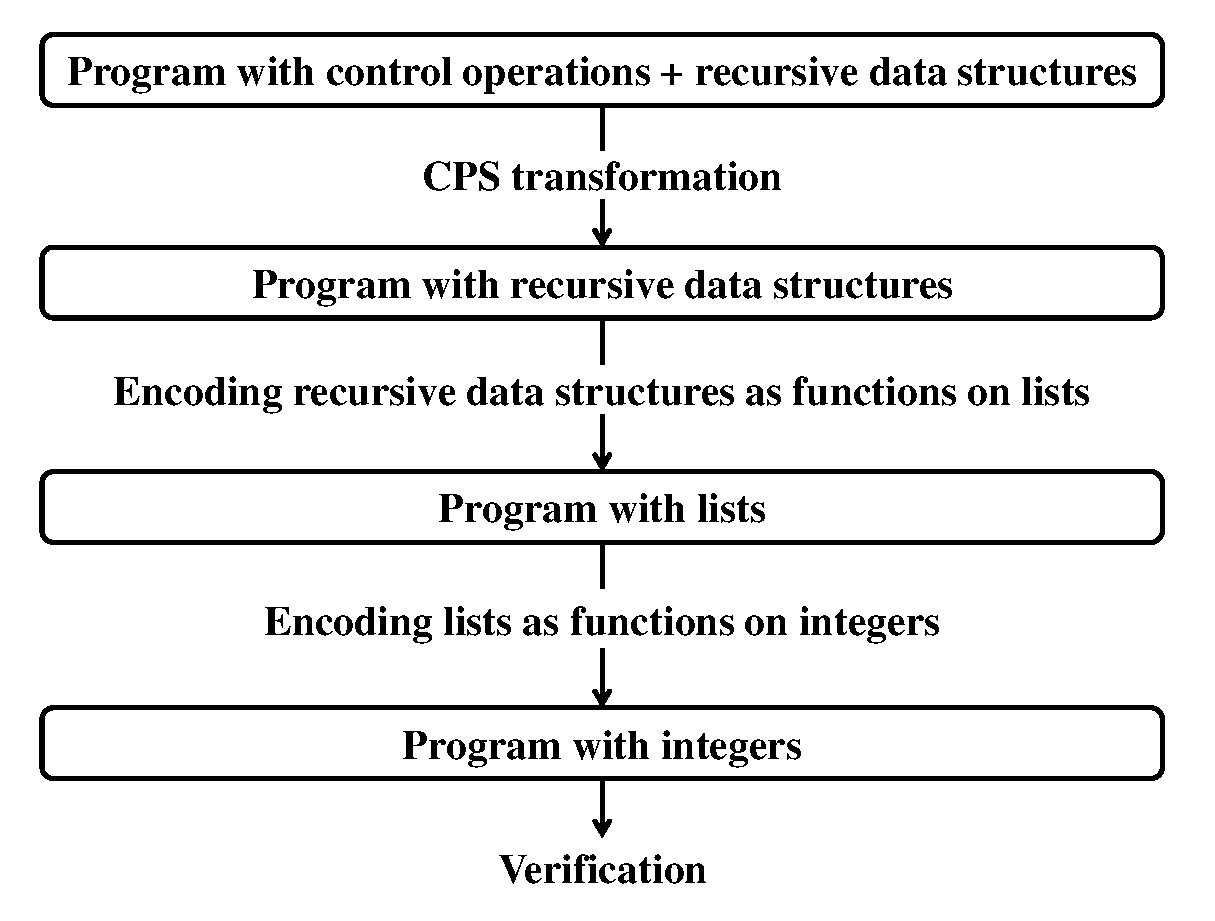
\includegraphics[scale=0.4]{extension.eps}
 \end{center}
\caption{The verification framework for recursive data structures and control operators}
\label{fig:extension}
\end{figure}

The Sect.~\ref{sec:recdata} formalizes the encoding of recursive data
structures, and Sect.~\ref{sec:control} introduces the extension for
control operations.

\subsection{Functional Encoding of Recursive Data Structures}
\label{sec:recdata}

In this section, we first formalize the encoding of lists, and then we discuss the
extension for user-defined recursive data structures.

%\[
%\begin{array}{lrl}
%D\text{ (programs)} &::=& \{f_1 = v_1, \dots, f_n = v_n\} \\
%t\text{ (terms)}
%  &::=& n \mid x \mid \Abs{x}{t} \mid t_1\ t_2 \mid \Op{v_1,\dots,v_n} \mid \If{t_1}{t_2}{t_3} \\
% &\mid& \FAIL \mid \Pair{v_1}{v_2} \mid \Fst{t} \mid \Snd{t} \mid \NIL \mid \Cons{v_1}{v_2} \\
% &\mid& (\MATCH\ {t_1}\ \WITH\ \NIL \ra {t_2} \mid \Cons{x_1}{x_2} \ra {t_3}) \\
%
%v\text{ (values)}
%  &::=& n \mid \Abs{x}{t} \mid \Pair{v_1}{v_2} \mid \NIL \mid \Cons{v_1}{v_2} \\
%
%E\text{ (eval. ctx.)}
%  &::=& [\,] \mid E\ t \mid \App{\Abs{x}{t}}{E} \mid \If{E}{t_2}{t_3} \mid \Fst{E} \mid \Snd{E} \\
% &\mid& (\Match{E}{t_2}{t_3}) \\
%
%\tau\text{ (types)} &::=& \INT \mid \TFun{\tau_1}{\tau_2} \mid \TPair{\tau_1}{\tau_2} \mid \List{\tau} \\
%\end{array}
%\]

%\begin{figure}[t]
%\begin{minipage}{\widthcoef\textwidth}
%\[
%\begin{array}{lrl}
%D\text{ (programs)} &::=& \{f_1 = v_1, \dots, f_n = v_n\} \\
%t\text{ (terms)}
%  &::=& n \mid x \mid \Abs{x}{t} \mid t_1\ t_2 \mid \Op{v_1,\dots,v_n} \mid \If{t_1}{t_2}{t_3} \\
% &\mid& \FAIL \mid \Pair{v_1}{v_2} \mid \Fst{t} \mid \Snd{t} \mid \NIL \mid \Cons{v_1}{v_2} \\
% &\mid& (\MATCH\ {t_1}\ \WITH\ \NIL \ra {t_2} \mid \Cons{x_1}{x_2} \ra {t_3}) \\
%
%v\text{ (values)}
%  &::=& n \mid \Abs{x}{t} \mid \Pair{v_1}{v_2} \mid \NIL \mid \Cons{v_1}{v_2} \\
%
%E\text{ (eval. ctx.)}
%  &::=& [\,] \mid E\ t \mid \App{\Abs{x}{t}}{E} \mid \If{E}{t_2}{t_3} \mid \Fst{E} \mid \Snd{E} \\
% &\mid& (\Match{E}{t_2}{t_3}) \\
%
%\tau\text{ (types)} &::=& \INT \mid \TFun{\tau_1}{\tau_2} \mid \TPair{\tau_1}{\tau_2} \mid \List{\tau} \\
%\end{array}
%\]
%\end{minipage}
%\caption{The syntax of source language with list}
%\label{fig:list-syntax}
%\end{figure}

\subsubsection{Functional Encoding of Lists}
\label{sec:list}

The idea is to encode a list into a pair of its length and a function that
maps indices to the elements of the list.  For example, the list
$[2;3;5]$ is encoded into the pair $(3,f)$ where $f(0) = 2$, $f(1) = 3$, and
$f(2) = 5$.  The primitive operations \texttt{nil}, \texttt{cons},
\texttt{is\_nil}, \texttt{head}, and \texttt{tail} for lists are defined
as follows.
\begin{alltt}
let nil = (0, fun _ -> fail)
let cons x (len,f) =
  let f' = if i = 0 then x else f (i-1) in (len+1, f')
let is_nil (len,f) = len = 0
let head (len,f) = if is_nil (len,f) then fail else f 0
let tail (len,f) =
  if is_nil (len,f) then fail else len-1, fun i -> f (i+1)
\end{alltt}
\texttt{nil} is translated into the pair of length $0$ and the
function that always fails.  \texttt{cons x xs} is translated into the
pair of its length and the function $\{0 \mapsto \mathtt{x}\} \cup \{i \mapsto
f (i-1) \mid i \neq 0\}$ where $f$ is the function part of encoding of
\texttt{xs}.  \texttt{is\_nil} just checks whether \texttt{len} is 0 or not.
\texttt{head} returns \texttt{f(0)}, i.e. the $0$-th
element of the list.  \texttt{tail} returns a pair of
\texttt{(len-1,f')} where $\mathtt{f'(i)} = \mathtt{f(i+1)}$.

%Since \texttt{f(i)} is the element whose position is \texttt{i} in the
%list, the encoded \texttt{head} returns \texttt{f(0)}, i.e. the $0$-th
%element of the list.  Function \texttt{tail} returns a pair of
%\texttt{(len-1,f')} where $\mathtt{f'(0)} = \mathtt{f(1)}$,
%$\mathtt{f'(1)} = \mathtt{f(2)}$, $\dots$

%Since the original \texttt{head} returns the head of a list,
%the encoded \texttt{head} returns the value

%consider the following
%program.
%\begin{alltt}
%let rec for_all p xs =
%  match xs with [] -> true
%          | x::xs' -> p x && for_all p xs'
%\end{alltt}
%\texttt{for\us{}all p [a1;...;an]} returns a boolean which represents
%whether \texttt{p(a$i$)} holds for every $i$.  We can obtain the
%following list-free program by the encoding mentioned above.
%\begin{alltt}
%let rec for_all p (len,f) =
%  if len = 0 then true
%  else let x = f 0 in
%       let len' = len - 1 in
%       let f' = fun i -> f (i+1) in
%         p x && for_all p (len',f')
%\end{alltt}
%The argument \texttt{xs} is translated into the pair of the length
%\texttt{len} and the function \texttt{f} such that \texttt{f($i$)}
%represents $i$-th element of the list \texttt{xs} (index is 1-origin.)
%The function \texttt{for\us{}all p}, which takes a list, is encoded to a
%higher-order function.  By this encoding, properties of lists are
%translated to ones of functions. For example, a property that
%\texttt{for\us{}all p xs} returns true, i.e. all the elements of
%\texttt{xs} satisfy \texttt{p}, is translated to a property that
%\texttt{f} always returns a positive integer.

This approach has the following advantages.  First, by encoding lists
into functions over integers, we can reuse the predicate
abstraction/discovery for integers.  Second, the encoding induces a
natural predicate abstraction of lists, which is general enough to
subsume various abstractions known in the literature, such as Dillig et
al.'s container abstraction~\cite{Dillig2011}.  In their abstraction
method for aggregate data structures like lists, a list is represented
as $\set{(v_1,P_1), \dots, (v_n,P_n)}$, a finite set of pairs of a
element of list and a condition for the index of the element.  For
example, $\set{(0,\TRUE)}$ denotes that all the elements are $0$ and
$\set{(1,\Abs{i}{i \mathop{\mathtt{mod}} 2 = 0})}$ denotes that the even
indexed elements are $1$.  On the other hand, by encoding a list as a
function, the same information can be represented as a refinement type
$\TFun{(i\COL\INT)}{\set{x\COL\INT\mid (P_1(i) \to x=v_1) \wedge \dots
\wedge (P_n(i) \to x=v_n)}}$.  For example, $\set{(1,\Abs{i}{i
\mathop{\mathtt{mod}} 2 = 0})}$ is represented as
$\TFun{(i\COL\INT)}{\set{x\COL\INT\mid i \mathop{\mathtt{mod}} 2 = 0 \to x=1}}$.  Moreover, our
approach can deal with list properties like ``the $i$-th
element of a list is greater than $i$,'' which cannot be represented by
the container abstraction.  Thus, our method, a combination of the encoding
and the predicate abstraction for integers, is strictly more powerful
than the container abstraction.

%\paragraph{Comparison with Dillig et al.'s appoach.}
%Dillig et al.~\cite{Dillig2011} have proposed an automatic technique for
%static reasoning about containers (e.g., maps, lists, and vectors). They
%model containers as functions that map a key to an abstract index that
%is mapped to a value corresponds to the index.  For example, a store
%includes list $[2;3]$ is abstracted as a map $\{\beta \mapsto
%\set{(\AbstLoc{\eta}{i}, \TRUE)}, \AbstLoc{\eta}{i} \mapsto
%\set{(2,i=0),(3,i=1),(\NIL,i \neq 0 \land i \neq 1)}\}$, where $\beta$
%is the memory location that stores the list, and $\AbstLoc{\eta}{i}$ is
%the abstract location indexed with $i$ that represents the list.  In the
%abstract store, $x \mapsto \set{(\pi_1, P_1), \dots, (\pi_n, P_n)}$
%represents that $x$ could have a value $\pi_i$ when $P_i$ holds.  Our
%approach is a generalization of their approach in the following sense:
%\begin{enumerate}
% \item While our abstraction uses arbitrary predicates for container elements,
%       they abstracts container elements to the set of unknown values,
%       integer constants, and locations.
% \item While our abstraction can depend on the index by the form ``if $P_(i)$
%       then $Q(i,v)$'' where $i$ is an index and $v$ is the element at the
%       index $i$, their abstraction can depend on the index only by the form ``if $P_(i)$
%       then $Q(v)$''.
%\end{enumerate}

%Once a target program is translated to a list-free program,
%we can apply our previous verification framework for higher-order programs with integers.

%Figure~\ref{fig:list-translation} shows the definition of the
%translation $\Trans{-}$.  Let $t$ be a list of the form
%$[v_0,\dots,v_{n-1}]$. $\Trans{t}$ denotes the pair of the length $n$ of
%$t$ and the function $\{0 \mapsto v_0, \dots, n-1 \mapsto v_{n-1}\}$
%that maps indices to elements of $t$.  $\NIL$ is translated into the pair of length $0$ and the
%function that always fails.  $\Cons{v_1}{v_2}$ is translated into the
%pair of its length and the function $\{0 \mapsto v_1\} \cup \{i \mapsto
%f (i-1) \mid i \neq 0\}$ where $f$ is the function part of encoding of
%$v_2$.  A pattern match is translated into an if-expression whose
%then-case and else-case respectively correspond to the $\NIL$ and
%$\Cons{x_1}{x_2}$ cases.
%
%\begin{figure}[t]
%\begin{minipage}{\widthcoef\textwidth}
%\[
%\begin{array}{l}
%% \Trans{n} = n \\
%% \Trans{x} = x \\
%% \Trans{\Fix{f}{x}{t}} = \Fix{f}{x}{\Trans{t}} \\
%% \Trans{t_1\ t_2} = \Trans{t_1}\ \Trans{t_2} \\
%% \Trans{\Op{v_1,\dots,v_n}} = \Op{\Trans{v_1}, \dots, \Trans{v_n}} \\
%% \Trans{\If{t_1}{t_2}{t_3}} = \If{\Trans{t_1}}{\Trans{t_2}}{\Trans{t_3}} \\
%% \Trans{\FAIL} = \FAIL \\
%% \Trans{\Pair{t_1}{t_2}} = \Pair{\Trans{t_1}}{\Trans{t_2}} \\
% \Trans{\NIL} = \Pair{0}{\Abs{u}{\FAIL}} \quad (\text{$u$ is fresh}) \\
%
% \Trans{\Cons{v_1}{v_2}} = (\Fst{v_2} + 1, \\
% \qquad \Abs{i}{\If{i-1}{\Trans{v_1}}{\Snd{v_2}\ (i-1)}}) \\
% \quad (\text{$i$ is fresh}) \\
%
% \Trans{\Match{t_1}{t_2}{t_3}} = \\
% \quad \Let{x}{\Trans{t_1}}{} \\
% \quad \Let{len}{\Fst{x}}{} \\
% \quad \Let{f}{\Snd{x}}{} \\
% \qquad \IF\ len\ \THEN\ \Trans{t_2} \\
% \qquad \ELSE\ \Let{x_1}{f\ 0}{}\\
% \qquad\qquad\, \Let{x_2}{\Pair{len - 1}{\Abs{i}{f (i+1)}}}{} \\
% \qquad\qquad\quad \Trans{t_3} \\
% \quad (\text{$x$, $len$, $f$ and $i$ are fresh}) \\
%\end{array}
%\]
%\end{minipage}
%\caption{Encoding of list (excerpt).}
%\label{fig:list-translation}
%\end{figure}

%The theorem below states that the translation $\Trans{-}$ is correct in
%the sense that if a source program fails, so does the translated program, and vice versa.
%\begin{theorem}[Correctness of translation]
%  \label{th:translation-list-correct}
%  Let $t$ be a term in a program $D$.
%  $t \Reds{D} \FAIL$ if and only if $\Trans{t} \Reds{D} \FAIL$.
%\end{theorem}



\subsubsection{Extension for Recursive Data Structures}
We discusses how to encode other recursive data structures.  We
translate programs with recursive data structures into programs with
lists by encoding recursive data structures to functions which map paths
of nodes to labels.  Here, a path and a label is represented as a list
of integers and an integer respectively.  Consider binary trees defined
as follows.
\begin{alltt}
type btree = Leaf | Node of btree * btree
\end{alltt}
A binary tree is encoded into a term of the type
$\TFun{\List\INT}{\INT}$.  For example, a binary tree
$\Node{\LEAF}{\Node{\LEAF}{\LEAF}}$ is encoded into a function $\{[]
\mapsto \NODE, [1] \mapsto \LEAF, [2] \mapsto \NODE, [2,1] \mapsto
\LEAF, [2,2] \mapsto \LEAF\}$ where $\LEAF$ and $\NODE$ are defined as
some integers.
Here is another example, the encoding of a pattern matching.
\begin{alltt}
match x with
  Constr_1(x1, x2, ...) -> t
| Constr_2 ...
\end{alltt}
The expression above is encoded to the following expression.
\begin{alltt}
let Constr_1 = 1 in
  ...
let Constr_n = n in
  match x nil with
    Constr_1 ->
      let x1 xs = x (cons 1 xs) in
      let x2 xs = x (cons 2 xs) in
        ...
      let xn xs = x (cons n xs) in
        t'
  | Constr_2 -> ...
\end{alltt}
Here, \texttt{t'} is the encoding of \texttt{t}. The pattern matching in
trees is translated to the pattern matching in labels, represented as
integers.  A subterm of a tree are obtained by adding the index to the head of the path.
%\begin{alltt}
%let rec get_child t =
%  match t with
%    Constr(t1,t2)Leaf -> fail
%  | Node(t1,t2) -> (t1, t2)
%\end{alltt}
%This program takes an unlabeled binary tree and returns its children.
%The program is translated into the following program with no recursive
%data structures except lists.
%\begin{alltt}
%let Leaf = 0
%let Node = 1
%let rec get_child t =
%  match t nil with
%    Leaf -> fail
%  | Node ->
%      let t1 xs = t (cons 0 xs) in
%      let t2 xs = t (cons 1 xs) in
%        (t1, t2)
%\end{alltt}

We treat only regular algebraic data types, i.e., the combination of sum
types and product types, which cannot have function types as arguments
of constructors.  We require that in a recursive type
$\RecType{\alpha}{\tau}$, $\alpha$ does not occur below function type
constructors. For example, $\List{\TFun{\INT}{\INT}}$ is OK, but neither
$\RecType{\alpha}{\TFun{\alpha}{\INT}}$ nor
$\RecType{\alpha}{\TFun{\INT}{\alpha}}$ is allowed.

%The reason is that the encoding recursive data types generates recursive types again.

%We introduce the language extended with recursive data structures.
%Figure~\ref{fig:rec-syntax} shows the syntax of the language.  The
%meta-variable $\CONSTR$ ranges over the sets of constructor names.
%$\Constr{}{v_1,\dots,v_k}$ is a constructor and $\MatchRec{t}{t_1}{t_k}$
%is a destructor for a type
%$\Constr{1}{\widetilde{\phi_1}} + \ldots + \Constr{k}{\widetilde{\phi_k}}$.
%A program is a pair of function definitions and type definitions
%$\gamma_1=\rho_1, \dots, \gamma_m=\rho_m$.
%A type definition
%$\gamma_1=\Constr{1}{\widetilde{\phi_1}} + \dots + \Constr{k}{\widetilde{\phi_k}}$
%means that type $\gamma$ has
%constructors $\CONSTR_1, \dots, \CONSTR_k$ and the types of the
%arguments of $C_i$ are $\widetilde{\phi_i}$.
%Note that, expressions for pattern matching on lists are distinct
%from ones for pattern matching on recursive data structures.  We restrict the types of the
%constructor arguments, represented by meta-variable $\phi$, to
%$\INT$ or recursive data types for the sake of simplicity.
%
%%We assume that $\gamma$ and $\CONSTR$ are distinct from others.
%
%
%\begin{figure}[t]
%\begin{minipage}{\textwidth}
%\[
%\begin{array}{lrl}
%D\text{ (program)} &::=& \{ f_1=t_1, \dots, f_n=t_n; \gamma_1=\rho_1, \ldots, \gamma_m=\rho_m \} \\
%t\text{ (terms)} &::=& \ldots \mid \Constr{}{\widetilde{v}} \mid (\MatchRec{t}{t_1}{t_k}) \\
%
%\rho\text{ (rec. type)} &::=& \Constr{1}{\widetilde{\phi_1}} + \dots + \Constr{k}{\widetilde{\phi_k}} \\
%\phi &::=& \INT \mid \gamma \\
%\tau\text{ (types)} &::=& \ldots \mid \gamma \\
%\end{array}
%\]
%\end{minipage}
%\caption{The syntax of language extended with recursive data structures}
%\label{fig:rec-syntax}
%\end{figure}
%
%\begin{example}
%A type definition for rose trees is represented as the following.
%\begin{eqnarray*}
% \RTREE &=& \RTNODE(\RTLIST) \\
% \RTLIST &=& \RTNIL() + \RTCONS(\RTREE, \RTLIST)
%\end{eqnarray*}
%%\memo{$\TREE = \NIL() + \NODE(\TREE, \TREE)$}
%\end{example}
%
%
%Figure~\ref{fig:rec-translation} shows the definitions of the translation $\TransRec{D}{-}$.
%$\TransRec{D}{t}$ denotes a function that maps paths to nodes of $t$.
%%Translation of constructors and destructors of lists are trivial, translate recursively.
%%We translate a recursive data $\Constr{}{v_1,\dots,v_n}$ into a function
%%that returns
%$\TransRec{D}{\Constr{}{v_1,\dots,v_n}}$ is a function that returns
%\begin{itemize}
% \item an integer $\TransRec{D}{C}$, correspondence number to $\CONSTR$, for $\NIL$,
% \item $v_k$ for a list whose head is $k$ when $v_k$ has type $\INT$, and
% \item $\App{\TransRec{D}{v_k}}{p}$ for a list that has the form of
%       $\Cons{k}{p}$ when $v_k$ has a recursive data type.
%\end{itemize}
%We translate $\MatchRec{t}{t_1}{t_k}$ into a if-expression that
%checks what is $\App{\TransRec{D}{t}}{\NIL}$, the root node label of
%$t$.  We can obtain the translated value%, the constructor
%argument, to which it bound to variable $x_{ij}$ by
%$\App{f}{(\Cons{i}{\NIL})}$ for $\INT$ and
%$\Abs{p}{\App{f}{(\Cons{i}{p})}}$ for recursive data types.
%%\TODO{add (or rewrite to) more intuitionistic explanation}




%\begin{figure}[t]
%\begin{minipage}{\textwidth}
%\[
%\begin{array}{l}
%% \TransRec{D}{n} = n \\
%% \TransRec{D}{x} = x \\
%% \TransRec{D}{\Fix{f}{x}{t}} = \Fix{f}{x}{\TransRec{D}{t}} \\
%% \TransRec{D}{t_1\ t_2} = \TransRec{D}{t_1}\ \TransRec{D}{t_2} \\
%% \TransRec{D}{\Op{t_1,\dots,t_n}} = \Op{\TransRec{D}{t_1}, \dots, \TransRec{D}{t_n}} \\
%% \TransRec{D}{\If{t_1}{t_2}{t_3}} = \If{\TransRec{D}{t_1}}{\TransRec{D}{t_2}}{\TransRec{D}{t_3}} \\
%% \TransRec{D}{\FAIL} = \FAIL \\
%% \TransRec{D}{\Pair{t_1}{t_2}} = \Pair{\TransRec{D}{t_1}}{\TransRec{D}{t_2}} \\
% \TransRec{D}{\NIL} = \NIL \\
% \TransRec{D}{\Cons{t_1}{t_2}} = \Cons{\TransRec{D}{t_1}}{\TransRec{D}{t_2}} \\
% \TransRec{D}{\Match{t_1}{t_2}{t_3}} = \\
%  \quad \Match{\TransRec{D}{t_1}}{\TransRec{D}{t_2}}{\TransRec{D}{t_3}} \\
%
% \TransRec{D}{\Constr{}{v_1,\dots,v_n}} = \\\qquad
%  \Abs{x}{}\MATCH\ x\ \WITH\ \NIL \ra \TransRec{D}{\CONSTR} \\\qquad\qquad
%  \begin{array}{ll}
%   \mid \Cons{k}{p} \ra & \If{k - 1}{\RecConstr{D}{C}{1}{p}{\TransRec{D}{v_1}}}{} \\
%                        & \If{k - 2}{\RecConstr{D}{C}{2}{p}{\TransRec{D}{v_2}}}{} \\
%                        & \quad \dots \\
%                        & \If{k - n}{\RecConstr{D}{C}{n}{p}{\TransRec{D}{v_n}}}{\FAIL} \\
%  \end{array} \\
% \TransRec{D}{\MatchRec{t}{t_1}{t_k}} = \\
% \quad \Let{f}{\TransRec{D}{t}}{} \\
% \quad \Let{l}{\App{f}{\NIL}}{} \\
% \qquad \If{l - 1}{\RecDestr{D}{\CONSTR_1}{f}{\TransRec{D}{t_1}}}{} \\
% \qquad \If{l - 2}{\RecDestr{D}{\CONSTR_2}{f}{\TransRec{D}{t_2}}}{} \\
% \qquad \quad \dots \\
% \qquad \If{l - k}{\RecDestr{D}{\CONSTR_k}{f}{\TransRec{D}{t_k}}}{\FAIL} \\
%\end{array}
%\]
%\[
%\begin{array}{l}
% \RecConstr{D}{\CONSTR}{k}{p}{v} =
%  \left\{
%  \begin{array}{ll}
%    v          & \quad \text{($\phi_k = \INT$)} \\
%    \App{v}{p} & \quad \text{(otherwise)}
%  \end{array}
%  \right. \\
%\qquad \text{where $D \ni (\gamma = \cdots + \Constr{}{\phi_1,\dots,\phi_j,\dots,\phi_n} + \cdots)$}
%
%%%% \begin{array}{rl}
%%%%   \RecDestr{D}{\gamma_i}{f}{j}{t} =
%%%%     & \Let{x_1}{\Abs{p}{f\ (\Cons{1}{p})}}{} \\
%%%%     & \dots \\
%%%%     & \Let{x_{n_i}}{\Abs{p}{f\ (\Cons{n_i}{p})}}{t}
%%%% \end{array} \\
%\end{array}
%\]
%
%\[
%\begin{array}{l}
% \begin{array}{rl}
%   \RecDestr{D}{\CONSTR}{f}{t} =
%     & \Let{x_1}{\RecDestrBase{D}{\CONSTR}{f}{1}}{} \\
%     & \quad \dots \\
%     & \Let{x_n}{\RecDestrBase{D}{\CONSTR}{f}{n}}{t}
% \end{array} \\
% \RecDestrBase{D}{\CONSTR}{f}{i} =
%  \left\{
%  \begin{array}{ll}
%    \App{f}{(\Cons{i}{\NIL})}       & \quad \text{($\phi_i = \INT$)} \\
%    \Abs{p}{\App{f}{(\Cons{i}{p})}} & \quad \text{(otherwise)}
%  \end{array}
%  \right. \\
%\qquad \text{where $D \ni (\gamma = \cdots + \Constr{}{\phi_1,\dots,\phi_i,\dots,\phi_n} + \cdots)$}
% \end{array}
%\]
%\end{minipage}
%\caption{Encoding of recursive data structures.
%$\TransRec{D}{\CONSTR}$ is an unique integer corresponds to $\CONSTR$.}
%\label{fig:rec-translation}
%\end{figure}

